% Do not forget to include Introduction
%---------------------------------------------------------------
% \chapter{Introduction}
% uncomment the following line to create an unnumbered chapter
\chapter*{Introduction}\addcontentsline{toc}{chapter}{Acknowledgments}\markboth{Introduction}{Introduction}
%---------------------------------------------------------------
\setcounter{page}{1}

% The following environment can be used as a mini-introduction for a chapter. Use that any way it pleases you (or comment it out). It can contain, for instance, a summary of the chapter. Or, there can be a quotation.
\begin{chapterabstract}
	\lipsum[1]
\end{chapterabstract}

\lipsum[2][1-4]{} [1]

\lipsum[4]

%---------------------------------------------------------------
\section{Ut enim ad minim veniam}
%---------------------------------------------------------------

\lipsum[6-7]

\begin{figure}
\centering
%\includegraphics[scale=0.4]{pic/index}
\resizebox{\textwidth}{!}{
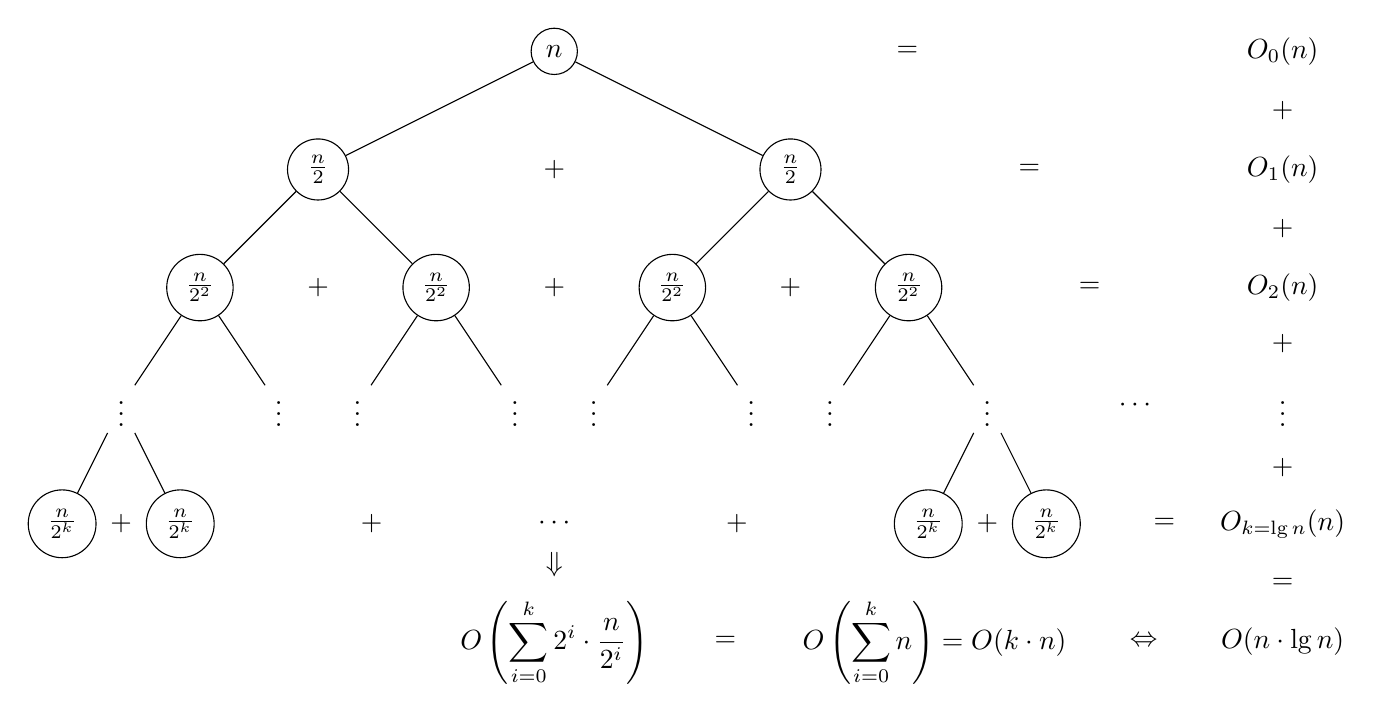
\begin{tikzpicture}[level/.style={sibling distance=60mm/#1}]
\node [circle,draw] (z){$n$}
  child {node [circle,draw] (a) {$\frac{n}{2}$}
    child {node [circle,draw] (b) {$\frac{n}{2^2}$}
      child {node {$\vdots$}
        child {node [circle,draw] (d) {$\frac{n}{2^k}$}}
        child {node [circle,draw] (e) {$\frac{n}{2^k}$}}
      } 
      child {node {$\vdots$}}
    }
    child {node [circle,draw] (g) {$\frac{n}{2^2}$}
      child {node {$\vdots$}}
      child {node {$\vdots$}}
    }
  }
  child {node [circle,draw] (j) {$\frac{n}{2}$}
    child {node [circle,draw] (k) {$\frac{n}{2^2}$}
      child {node {$\vdots$}}
      child {node {$\vdots$}}
    }
  child {node [circle,draw] (l) {$\frac{n}{2^2}$}
    child {node {$\vdots$}}
    child {node (c){$\vdots$}
      child {node [circle,draw] (o) {$\frac{n}{2^k}$}}
      child {node [circle,draw] (p) {$\frac{n}{2^k}$}
        child [grow=right] {node (q) {$=$} edge from parent[draw=none]
          child [grow=right] {node (q) {$O_{k = \lg n}(n)$} edge from parent[draw=none]
            child [grow=up] {node (r) {$\vdots$} edge from parent[draw=none]
              child [grow=up] {node (s) {$O_2(n)$} edge from parent[draw=none]
                child [grow=up] {node (t) {$O_1(n)$} edge from parent[draw=none]
                  child [grow=up] {node (u) {$O_0(n)$} edge from parent[draw=none]}
                }
              }
            }
            child [grow=down] {node (v) {$O(n \cdot \lg n)$}edge from parent[draw=none]}
          }
        }
      }
    }
  }
};
\path (a) -- (j) node [midway] {+};
\path (b) -- (g) node [midway] {+};
\path (k) -- (l) node [midway] {+};
\path (k) -- (g) node [midway] {+};
\path (d) -- (e) node [midway] {+};
\path (o) -- (p) node [midway] {+};
\path (o) -- (e) node (x) [midway] {$\cdots$}
  child [grow=down] {
    node (y) {$O\left(\displaystyle\sum_{i = 0}^k 2^i \cdot \frac{n}{2^i}\right)$}
    edge from parent[draw=none]
  };
\path (q) -- (r) node [midway] {+};
\path (s) -- (r) node [midway] {+};
\path (s) -- (t) node [midway] {+};
\path (s) -- (l) node [midway] {=};
\path (t) -- (u) node [midway] {+};
\path (z) -- (u) node [midway] {=};
\path (j) -- (t) node [midway] {=};
\path (y) -- (x) node [midway] {$\Downarrow$};
\path (v) -- (y)
  node (w) [midway] {$O\left(\displaystyle\sum_{i = 0}^k n\right) = O(k \cdot n)$};
\path (q) -- (v) node [midway] {=};
\path (e) -- (x) node [midway] {+};
\path (o) -- (x) node [midway] {+};
\path (y) -- (w) node [midway] {$=$};
\path (v) -- (w) node [midway] {$\Leftrightarrow$};
\path (r) -- (c) node [midway] {$\cdots$};
\end{tikzpicture}}
\caption{~Lorem ipsum dolor sit amet}\label{img:index}
\end{figure}

%---------------------------------------------------------------
\section{Ut enim ad minim veniam}
%---------------------------------------------------------------

\lipsum[2-4]

%---------------------------------------------------------------
\subsection{Ut enim ad minim veniam}
%---------------------------------------------------------------

Curabitur ligula sapien, pulvinar a vestibulum quis, facilisis vel sapien. Duis condimentum augue id magna semper rutrum. Aliquam ornare wisi eu metus. Fusce aliquam vestibulum ipsum. Vivamus ac leo pretium faucibus\ref{img:index}.

\begin{itemize}
    \item Ut enim ad minim veniam, quis nostrud
    \item Ut enim ad minim 
    \item Ut enim ad minim veniam, quis 
    \begin{itemize}
        \item Ut enim ad
        \item Ut enim ad
        \begin{itemize}
            \item Ut enim 
            \item Ut enim 
            \begin{itemize}
            \item Ut enim 
            \item Ut enim 
        \end{itemize}
        \end{itemize}
    \end{itemize}
\end{itemize}

\section{Class aptent taciti}

\lipsum[2]

\subsection{Class aptent taciti}

\lipsum[6-7]

\begin{enumerate}
    \item Ut enim ad minim veniam, quis nostrud
    \item Ut enim ad minim 
    \item Ut enim ad minim veniam, quis 
    \begin{enumerate}
        \item Ut enim ad
        \item Ut enim ad
        \begin{enumerate}
            \item Ut enim 
            \item Ut enim 
            \begin{enumerate}
            \item Ut enim 
            \item Ut enim 
        \end{enumerate}
        \end{enumerate}
    \end{enumerate}
\end{enumerate}


%---------------------------------------------------------------
\section{Ut enim ad minim veniam, quis nostrud}
%---------------------------------------------------------------

Ut enim ad minim veniam, quis nostrud exercitation ullamco laboris nisi ut aliquip ex ea commodo consequat. Nulla non arcu lacinia neque faucibus fringilla. Vestibulum erat nulla, ullamcorper nec, rutrum non, nonummy ac, erat. Aliquam erat volutpat. Proin pede metus, vulputate nec, fermentum fringilla, vehicula vitae, justo.\footnote{Ut enim ad minim veniam, quis nostrud exercitation.} Etiam dictum tincidunt diam. In laoreet, magna id viverra tincidunt, sem odio bibendum justo, vel imperdiet sapien wisi sed libero. Nulla est. Maecenas fermentum, sem in pharetra pellentesque, velit turpis volutpat ante, in pharetra metus odio a lectus. Duis aute irure dolor in reprehenderit in voluptate velit esse cillum dolore eu fugiat nulla pariatur. 

%\begin{lstlisting}[caption={~Zbytečný kód},label=list:8-6,captionpos=t,float,abovecaptionskip=-\medskipamount,belowcaptionskip=\medskipamount,language=C]
%    #include<stdio.h>
%    #include<iostream>
%    // A comment
%    int main(void)
%    {
%        printf("Hello World\n");
%        return 0;
%    }
%\end{lstlisting}

%%%%%%%%%%%%%%%%%%%%%%%%%%%%%%%%%
% alternative using package minted for source highlighting
% package minted requires execution with `-shell-escape'
% e.g., `xelatex -shell-escape ctufit-thesis.tex'
 \begin{listing}
 \caption{Zbytečný kód}\label{list:8-6}
 \begin{minted}{C}
     #include<stdio.h>
     #include<iostream>
     // A comment
     int main(void)
     {
         printf("Hello World\n");
         return 0;
     }
 \end{minted}
 \end{listing}
% %%%%%%%%%%%%%%%%%%%%%%%%%%%%%%%%%

Nullam feugiat, turpis at pulvinar vulputate, erat libero tristique tellus, nec bibendum odio risus sit amet ante. Aenean id metus id velit ullamcorper pulvinar. Fusce wisi. Integer lacinia. Aliquam id dolor. Pellentesque pretium lectus id turpis. Suspendisse sagittis ultrices augue. In laoreet, magna id viverra tincidunt, sem odio bibendum justo, vel imperdiet sapien wisi sed libero. Sed ac dolor sit amet purus malesuada congue. \cite{Crochemore2002}

Class aptent taciti sociosqu ad litora torquent per conubia nostra, per inceptos hymenaeos. Fusce suscipit libero eget elit. Etiam dui sem, fermentum vitae, sagittis id, malesuada in, quam. Aliquam id dolor. Curabitur bibendum justo non orci. Duis viverra diam non justo. Curabitur ligula sapien, pulvinar a vestibulum quis, facilisis vel sapien. Duis condimentum augue id magna semper rutrum. Aliquam ornare wisi eu metus. Fusce aliquam vestibulum ipsum. Vivamus ac leo pretium faucibus. \cite{Motwani2014}

%---------------------------------------------------------------
\subsection{Ut enim ad minim veniam, quis nostrud}
%---------------------------------------------------------------

Ut enim ad minim veniam, quis nostrud exercitation ullamco laboris nisi ut aliquip ex ea commodo consequat. Nulla non arcu lacinia neque faucibus fringilla. Vestibulum erat nulla, ullamcorper nec, rutrum non, nonummy ac, erat. Aliquam erat volutpat. Proin pede metus, vulputate nec, fermentum fringilla, vehicula vitae, justo. Etiam dictum tincidunt diam. In laoreet, magna id viverra tincidunt, sem odio bibendum justo. \cite{Sestakova2018} 

\begin{table}\centering
\caption[Příklad tabulky]{~Zadávání matematiky}\label{tab:matematika}
\begin{tabular}{l|l|c|c}
	Typ		& Prostředí		& \LaTeX{}ovská zkratka	& \TeX{}ovská zkratka	\tabularnewline \hline 
 	Text		& \verb|math|		& \verb|\(...\)|	& \verb|$...$|	\tabularnewline \hline
 	Displayed	& \verb|displaymath|	& \verb|\[...\]|	& \verb|$$...$$|	\tabularnewline 
\end{tabular}
\end{table}


Nulla est. Maecenas fermentum, sem in pharetra pellentesque, velit turpis volutpat ante, in pharetra metus odio a lectus. Duis aute irure dolor in reprehenderit in voluptate velit esse cillum dolore eu fugiat nulla pariatur. Nullam feugiat, turpis at pulvinar vulputate, erat libero tristique tellus, nec bibendum odio risus sit amet ante. Aenean id metus id velit ullamcorper pulvinar. 

\subsubsection{Class aptent taciti}

\begin{definition}[Optional label]
Class aptent taciti sociosqu ad litora torquent per conubia nostra, per inceptos hymenaeos. Fusce suscipit libero eget elit. Etiam dui sem, fermentum vitae, sagittis id, malesuada in, quam. Aliquam id dolor. Curabitur bibendum justo non orci.
\end{definition}

\begin{example}
Class aptent taciti sociosqu ad litora torquent per conubia nostra, per inceptos hymenaeos. Fusce suscipit libero eget elit. Etiam dui sem, fermentum vitae, sagittis id, malesuada in, quam. Aliquam id dolor. Curabitur bibendum justo non orci.
\end{example}

\begin{theorem}
Class aptent taciti sociosqu ad litora torquent per conubia nostra, per inceptos hymenaeos. Fusce suscipit libero eget elit. Etiam dui sem, fermentum vitae, sagittis id, malesuada in, quam. Aliquam id dolor. Curabitur bibendum justo non orci.
\end{theorem}

\begin{proof}
Fusce suscipit libero eget elit. Etiam dui sem, fermentum vitae, sagittis id, malesuada in, quam. Aliquam id dolor. Curabitur bibendum justo non orci.
\end{proof}

\begin{corollary}
Fusce suscipit libero eget elit. Etiam dui sem, fermentum vitae, sagittis id, malesuada in, quam. Aliquam id dolor. Curabitur bibendum justo non orci.
\end{corollary}

\begin{proposition}
Fusce suscipit libero eget elit. Etiam dui sem, fermentum vitae, sagittis id, malesuada in, quam. Aliquam id dolor. Curabitur bibendum justo non orci.
\end{proposition}

\begin{note}
Fusce suscipit libero eget elit. Etiam dui sem, fermentum vitae, sagittis id, malesuada in, quam. Aliquam id dolor. Curabitur bibendum justo non orci.
\end{note}

\begin{remark}
Fusce suscipit libero eget elit. Etiam dui sem, fermentum vitae, sagittis id, malesuada in, quam. Aliquam id dolor. Curabitur bibendum justo non orci.
\end{remark}

\begin{lemma}
Class aptent taciti sociosqu ad litora torquent per conubia nostra, per inceptos hymenaeos. Fusce suscipit libero eget elit. Etiam dui sem, fermentum vitae, sagittis id, malesuada in, quam. Aliquam id dolor. Curabitur bibendum justo non orci.
\end{lemma}

\lipsum[1-2]

\subsection{Class aptent taciti sociosqu}

\lipsum[4-5]

%---------------------------------------------------------------
\chapter{Binární halda}
%---------------------------------------------------------------

\begin{figure}[H]
	\centering
	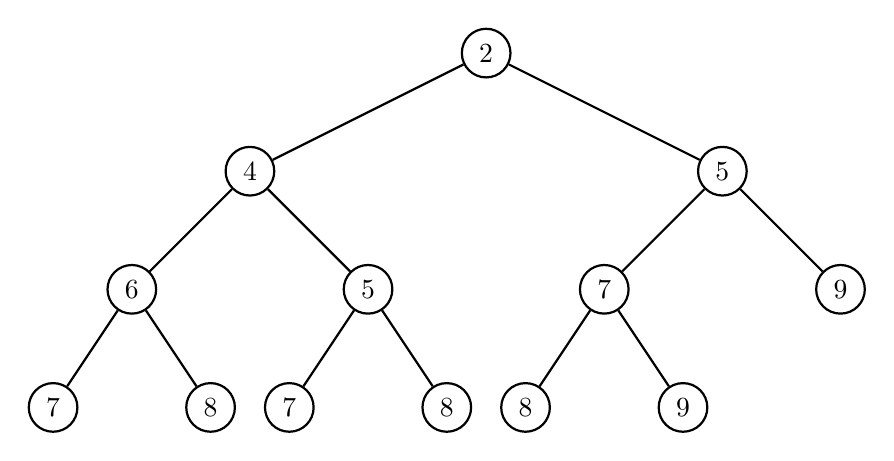
\begin{tikzpicture}[level/.style={sibling distance=60mm/#1}]
		\node [circle,draw,thick] (0) {2}
		child[thick] { node [circle,draw] (1) {4}
			child { node [circle,draw] (3) {6}
				child { node [circle,draw] (7) {7} }
				child { node [circle,draw] (8) {8} }
			}
			child { node [circle,draw] (4) {5}
				child { node [circle,draw] (9) {7} }
				child { node [circle,draw] (10) {8} }
			}
		}
		child[thick] { node [circle,draw] (2) {5}
			child { node [circle,draw] (5) {7}
				child { node [circle,draw] (11) {8} }
				child { node [circle,draw] (12) {9} }
			}
			child {node [circle,draw] (6) {9} }
		};
	\end{tikzpicture}
	\caption{~Lorem ipsum dolor sit amet}\label{img:index2}
\end{figure}

\begin{definition}[Uložení haldy v poli]
...
\end{definition}


%---------------------------------------------------------------
\chapter{Implementace důkazu binární haldy}
%---------------------------------------------------------------

Lorem ipsum dolor sit amet, consectetuer adipiscing elit. Curabitur sagittis hendrerit ante. Class aptent taciti sociosqu ad litora torquent per conubia nostra, per inceptos hymenaeos. Cras pede libero, dapibus nec, pretium sit amet, tempor quis. Sed vel lectus. Donec odio tempus molestie, porttitor ut, iaculis quis, sem. Suspendisse sagittis ultrices augue. Donec ipsum massa, ullamcorper in, auctor et, scelerisque sed, est. In sem justo, commodo ut, suscipit at, pharetra vitae, orci. Pellentesque pretium lectus id turpis.

\section{Hledání minimálního prvku}

\section{Probublání prvku nahoru}
\label{subsec:HeapBubbleUp}

Probublání prvku haldy směrem nahoru (ke kořeni) je operace nad haldou, která dokáže v čase $\mathcal{O}(\log(n))$ opravit haldové uspořádání za předpokladu, že se snížila hodnota pouze toho vrcholu, který má být probublán.

Algoritmus předpokládá, že haldové uspořádání je možné porušit pouze mezi jednou dvojicí vrcholů $u$ a $v$, kde $u$ je rodičovský vrchol a $v$ je jeho potomek. Tedy v celé haldě s výjimkou této dvojice musí platit haldové uspořádání. V této dvojici může platit, že syn~$v$ má menší hodnotu než jeho otec~$u$. Dále se předpokládá, že tento algoritmus bude proveden po zmenšení hodnoty některého vrcholu nebo po vložení nového vrcholu do haldy. V obou případech je potřeba tento vrchol probublat nahoru do správné pozice v haldě. Pokud by se hodnota zvýšila, měl by být aplikován algoritmus probublání dolů, o kterém pojednává sekce \ref{subsec:HeapBubbleDown}.

\begin{listing}[H]
	\caption{Probublání prvku nahoru}
	\label{list:HeapBubbleUp}
	\begin{minted}{c}
void HeapBubbleUp(Heap heap, int index) {
  int parent;

  while (HeapHasParent(heap, index)) {
    parent = HeapParent(index);

    if (HeapElementValue(heap, parent) <= HeapElementValue(heap, index)) {
      break;
    }

    HeapSwap(heap, index, parent);

    index = parent;
  }
}
	\end{minted}
\end{listing}

Pro důkaz korektnosti tohoto algoritmu jsou použity \textit{řezy} haldou. Tyto řezy slouží pro rozdělení grafu haldy na dva podgrafy, ve kterých platí haldové uspořádání. Řezy dohromady tvoří původní graf haldy bez jedné problematické hrany $(u, v)$, ve které nemusí platit haldové uspořádání.

Rozdělení haldy pro operaci probublání nahoru by mohlo vypadat podobně jak znázorňuje Obrázek \ref{img:heap-intuitive-cut}. Tento přístup ale není vhodný pro algoritmické zpracování a dokazovaní, jelikož se toto rozdělení složitě popisuje. Zavedeme proto horní a spodní řezy haldy pomocí potomka, které pracují s indexy jednotlivých prvků haldy reprezentované polem.

\begin{figure}[H]
	\centering
	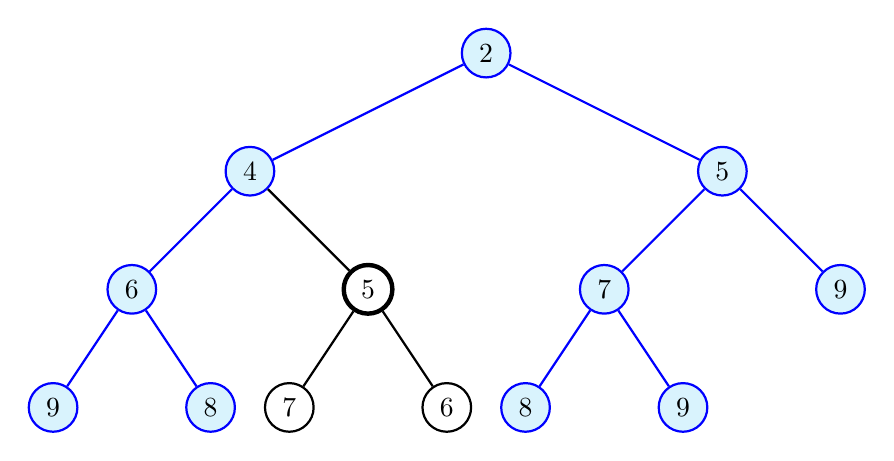
\begin{tikzpicture}[level/.style={sibling distance=60mm/#1}]
		\node [circle,thick,draw=blue,fill=cyan!15] (0) {2}
		child[thick,draw=blue] { node [circle,draw,fill=cyan!15] (1) {4}
			child { node [circle,draw,fill=cyan!15] (3) {6}
				child { node [circle,draw,fill=cyan!15] (7) {9} }
				child { node [circle,draw,fill=cyan!15] (8) {8} }
			}
			child[draw=black] { node [circle,draw,ultra thick] (4) {5}
				child { node [circle,draw] (9) {7} }
				child { node [circle,draw] (10) {6} }
			}
		}
		child[thick,draw=blue] { node [circle,draw,fill=cyan!15] (2) {5}
			child { node [circle,draw,fill=cyan!15] (5) {7}
				child { node [circle,draw,fill=cyan!15] (11) {8} }
				child { node [circle,draw,fill=cyan!15] (12) {9} }
			}
			child { node [circle,draw,fill=cyan!15] (6) {9} }
		};
	\end{tikzpicture}
	\caption{Ukázka intuitivního řezu haldy}
	\label{img:heap-intuitive-cut}
\end{figure}

\begin{definition}[Vrchní řez haldy pomocí potomka]
	Mějme graf $G = (V, E)$ reprezentující binární haldu a~$i \in \mathbb{N}$.
	Vrchním řezem haldy pomocí potomka nazveme graf $G' = (V', E')$, kde
	\begin{enumerate}
	  \item[] $V' = \{ v: v \in V \land \Index(v) < i \}$
	  \item[] $E' = \{ (u, v): (u, v) \in E \land u \in V' \land v \in V' \}$.
	\end{enumerate}
\end{definition}

\begin{figure}[H]
	\centering
	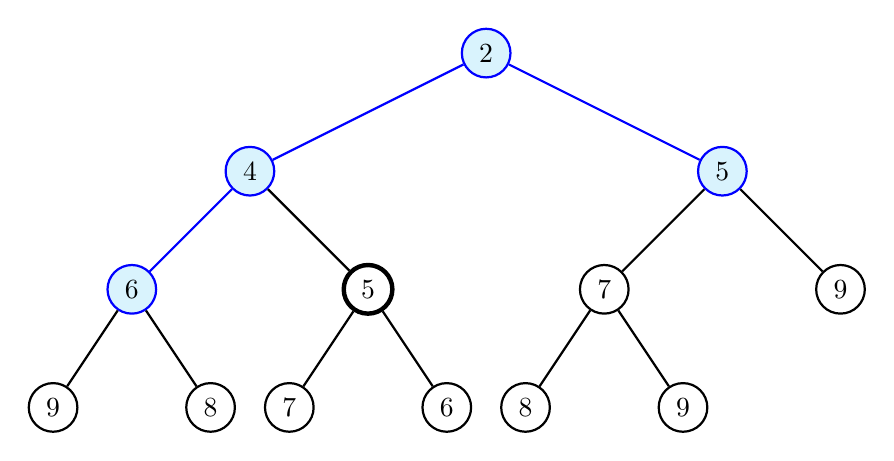
\begin{tikzpicture}[level/.style={sibling distance=60mm/#1}]
		\node [circle,thick,draw=blue,fill=cyan!15] (0) {2}
		child[thick,draw=blue] { node [circle,draw,fill=cyan!15] (1) {4}
			child { node [circle,draw,fill=cyan!15] (3) {6}
				child[draw=black] { node [circle,draw] (7) {9} }
				child[draw=black] { node [circle,draw] (8) {8} }
			}
			child[draw=black] { node [circle,draw,ultra thick] (4) {5}
				child { node [circle,draw] (9) {7} }
				child { node [circle,draw] (10) {6} }
			}
		}
		child[thick,draw=blue] { node [circle,draw,fill=cyan!15] (2) {5}
			child[draw=black] { node [circle,draw] (5) {7}
				child { node [circle,draw] (11) {8} }
				child { node [circle,draw] (12) {9} }
			}
			child[draw=black] {node [circle,draw] (6) {9} }
		};
	\end{tikzpicture}
	\caption{Ukázka vrchního řezu haldy pomocí potomka}
	\label{img:heap-upper-child-cut}
\end{figure}

\begin{remark}
	V grafu vrchního řezu haldy pomocí potomka platí haldové uspořádání.
\end{remark}

ACSL kód popisující vrchní řez haldy pomocí potomka nevytváří nový podgraf s~výše definovanými vlastnostmi, ale pouze ověřuje, že daná část (podgraf) haldy splňuje haldové uspořádání. Takto vytvořený predikát je následně použit v kontraktu funkce jako jedna ze vstupních podmínek algoritmu probublání nahoru a je také použit jako invariant cyklu. Predikát je tedy platný při volání funkce, po každém kroku cyklu a je také platný na konci vykonávání funkce. Nemusí ale platit, že je graf vrchního řezu haldy na konci vykonávání funkce prázdný. Tato situace by nastala pouze v případě, že byl problematický vrchol probublán až do kořene haldy. Tato induktivní vlastnost následně napomáhá při dokončení důkazu korektnosti algoritmu probublání nahoru.

\begin{listing}[H]
	\caption{Predikát validního vrchního řezu v haldě pomocí potomka}
	\label{acsl:HeapUpperChildCut}
	\begin{minted}{c}
/*@
  predicate HeapUpperChildCut(Heap heap, integer index) =
    \forall integer ancestor, descendant;
      0 <= ancestor < descendant < HeapElementsCount(heap)
      && descendant < index
      && IsParent(ancestor, descendant) ==>
        HasHeapProperty(heap, ancestor, descendant);
*/
	\end{minted}
\end{listing}

\begin{definition}[Spodní řez haldy pomocí potomka]
	Mějme graf $G = (V, E)$ reprezentující binární haldu a~$i \in \mathbb{N}$.
	Spodním řezem haldy pomocí potomka nazveme graf $G' = (V', E')$, kde
	\begin{enumerate}
	  \item[] $V' = \{ v: v \in V \land \Index(v) > i \} \cup \{ \Parent(v): v \in V \land \Index(v) > i \}$
	  \item[] $E' = \{ (u, v): (u, v) \in E \land u \in V' \land v \in V' \}$.
	\end{enumerate}
\end{definition}

\begin{figure}[H]
	\centering
	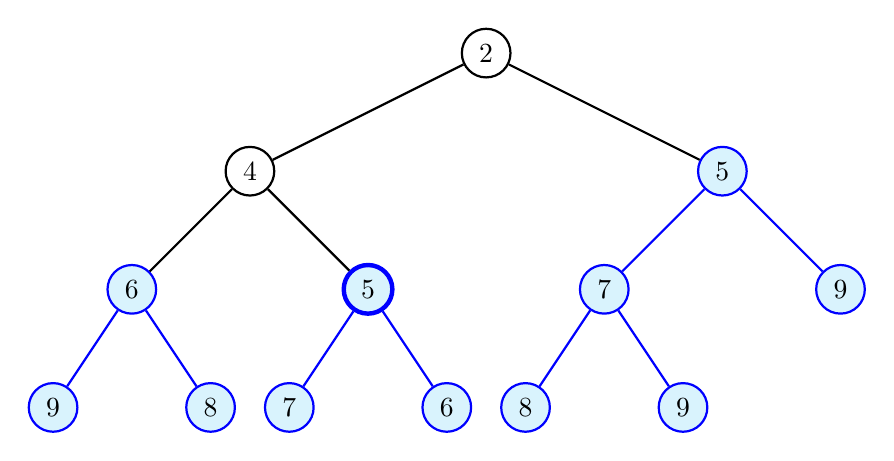
\begin{tikzpicture}[level/.style={sibling distance=60mm/#1}]
		\node [circle,thick,draw] (0) {2}
		child[thick] { node [circle,draw] (1) {4}
			child { node [circle,draw=blue,fill=cyan!15] (3) {6}
				child[draw=blue] { node [circle,draw,fill=cyan!15] (7) {9} }
				child[draw=blue] { node [circle,draw,fill=cyan!15] (8) {8} }
			}
			child { node [circle,draw=blue,fill=cyan!15,ultra thick] (4) {5}
				child[draw=blue] { node [circle,draw,fill=cyan!15] (9) {7} }
				child[draw=blue] { node [circle,draw,fill=cyan!15] (10) {6} }
			}
		}
		child[thick] { node [circle,draw=blue,fill=cyan!15] (2) {5}
			child[draw=blue] { node [circle,draw,fill=cyan!15] (5) {7}
				child { node [circle,draw,fill=cyan!15] (11) {8} }
				child { node [circle,draw,fill=cyan!15] (12) {9} }
			}
			child[draw=blue] {node [circle,draw,fill=cyan!15] (6) {9} }
		};
	\end{tikzpicture}
	\caption{Ukázka spodního řezu haldy pomocí potomka}\label{img:heap-lower-child-cut}
\end{figure}

\begin{remark}
	V grafu spodního řezu haldy pomocí potomka platí haldové uspořádání.
\end{remark}

ACSL implementace predikátu pro spodní řez haldy pomocí potomka je velmi podobná hornímu řezu. Oproti vrchnímu řezu, který pokrývá vrcholy haldy s indexem menším než problematický vrchol, spodní řez pokrývá potomky s vyšším indexem než problematický vrchol.

\begin{listing}[H]
	\caption{Predikát validního spodního řezu v haldě pomocí potomka}
	\label{acsl:HeapLowerChildCut}
	\begin{minted}{c}
/*@
  predicate HeapLowerChildCut(Heap heap, integer index) =
    \forall integer ancestor, descendant;
      0 <= ancestor < descendant < HeapElementsCount(heap)
      && index < descendant
      && IsParent(ancestor, descendant) ==>
        HasHeapProperty(heap, ancestor, descendant);
*/
	\end{minted}
\end{listing}

Výpis kódu \ref{acsl:HeapLowerChildCut} správně odděluje vrcholy, které mají index vyšší než problematický vrchol. Zároveň ale neomezuje hodnoty rodičovských vrcholů. Proto se do spodního řezu pomocí potomka správně dostane i problematický vrchol a také rodičovské vrcholy, které mají menší index než problematický vrchol. Hrana mezi problematickým vrcholem a jeho rodičovským vrcholem zde správně není.

Poslední nutnou vlastností pro úspěšné dokončení důkazu je tranzitivní haldové uspořádání mezi vrchním a spodním řezem haly. Tato vlastnost je automaticky splněna pro všechny hrany s výjimkou hrany, na které leží problematický vrchol v roli potomka. Proto do kódu zavádíme vstupní podmínku a invariantu cyklu, které kontrolují, zda platí haldové uspořádání pro rodičovský vrchol problematického vrcholu a jednotlivé potomky problematického vrcholu.

Tato vlastnost umožňuje probublávat problematický vrchol nahoru, zaručuje totiž, že rodičovský prvek, který s problematickým vrcholem vyměníme, bude po provedení výměny splňovat haldové uspořádání se svými novými potomky.

\begin{listing}[H]
	\caption{Predikáty tranzitivního haldového uspořádání mezi řezy haldou}
	\begin{minted}{c}
/*@
  predicate HeapLowerChildCutHeapPropertyLeftChild(Heap heap, integer index) = 
    HeapHasParent(heap, index)
    && HeapHasLeftChild(heap, index) ==>
      HasHeapProperty(heap, Parent(index), LeftChild(index));

  predicate HeapLowerChildCutHeapPropertyRightChild(Heap heap, integer index) =
    HeapHasParent(heap, index)
    && HeapHasRightChild(heap, index) ==>
      HasHeapProperty(heap, Parent(index), RightChild(index));
*/
	\end{minted}
\end{listing}

Platnost těchto čtyř invariantů dokazuje, že algoritmus probublání nahoru vždy vytváří maximálně jednu novou problematickou dvojici vrcholů. Haldové uspořádání mezi touto dvojicí vrcholů je opraveno probubláním na správnou pozici nebo úplným probubláním vrcholu do kořene haldy.

Spojením horního a spodního řezu haldou a tranzitivního haldového uspořádání je možné formálně dokázat korektnost algoritmu probublání prvku nahoru. Jelikož tyto vlastnosti platí na konci každého kroku cyklu, po dokončení cyklu se nacházíme v jednom z těchto stavů:

\begin{enumerate}
  \item problematický prvek probublal až do kořene haldy,
  \item problematický prvek nemohl dále probublat, tudíž je na správné pozici v haldě.
\end{enumerate}

Oba případy nám při spojení znalostí o horním a dolním řezu haldou a znalostí o aktuálně opravené hraně dávají výsledek, že pro každou hranu $(u, v)$ haldy, kde $u$ je rodičovský vrchol $v$, platí haldové uspořádání.

\begin{figure}[H]
	\centering
	\includegraphics[width=10cm]{images/frama-c-BubbleUp}
	\caption{Úspešné dokončení důkazu v prostředí Frama-C}
	\label{img:F-C-HeapBubbleUp}
\end{figure}

\section{Vložení prvku}
\label{subsec:HeapInsert}

Vložení prvku do haldy je operace nad haldou, která v čase $\mathcal{O}(1)$ vkládá nový vrchol do haldy a následně v~čase $\mathcal{O}(\log(n))$ tento vrchol umisťuje na správnou pozici v haldě. Celková asymptotická časová složitost je tedy $\mathcal{O}(\log(n))$.

Algoritmus přidává nový vrchol do nejspodnější hladiny haldy tak, aby byl udržen tvar haldy. Pro takto vložený vrchol ale nemusí platit haldové uspořádání s jeho rodičovským vrcholem. Haldové uspořádání před vložením vrcholu platilo pro všechny vrcholy s nižším indexem, než má aktuálně přidaný prvek. Zároveň se mohlo stát, že byl vložen vrchol s menší hodnotou než má jeho rodičovský vrchol. Proto je nutné provést probublání nahoru, o kterém pojednává sekce \ref{subsec:HeapBubbleUp}.

Algoritmus probublání vrcholu nahoru má tří vstupní podmínky. V haldě musí platit predikát o horním řezu podle potomka, který v případě přidání nového vrcholu platí. Před přidáním jsme měli haldu, kde platilo haldové uspořádání. Nový prvek je vložen na nový největší index v haldě. Tedy pro tento nový index platí řez haldou pomocí potomka, protože tento řez popisuje původní graf haldy. Spodní řez haldy pomocí potomka také platí, protože je to prázdný graf. Tranzitivní haldové uspořádání u aktuálně přidaného vrcholu také platí, jelikož tento vrchol nemá žádné potomky.

\begin{figure}[H]
	\centering
	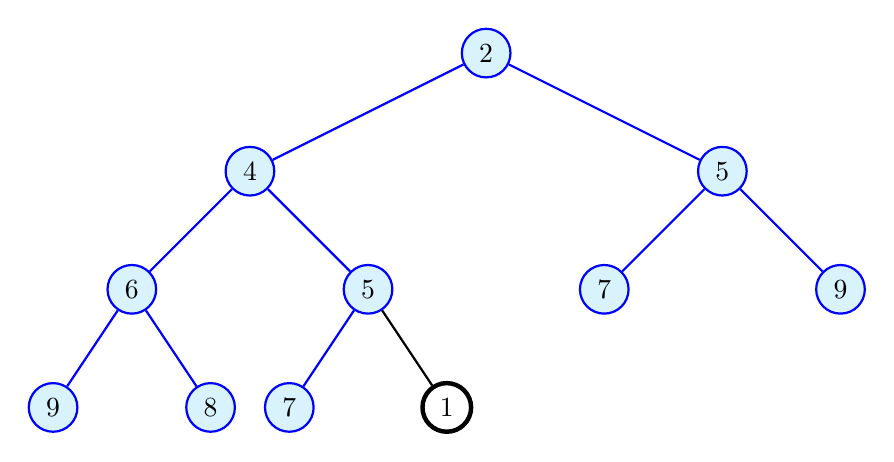
\begin{tikzpicture}[level/.style={sibling distance=60mm/#1}]
		\node [circle,thick,draw=blue,fill=cyan!15] (0) {2}
		child[thick,draw=blue] { node [circle,draw,fill=cyan!15] (1) {4}
			child { node [circle,draw,fill=cyan!15] (3) {6}
				child { node [circle,draw,fill=cyan!15] (7) {9} }
				child { node [circle,draw,fill=cyan!15] (8) {8} }
			}
			child { node [circle,draw,,fill=cyan!15] (4) {5}
				child { node [circle,draw,fill=cyan!15] (9) {7} }
				child[draw=black] { node [circle,draw,ultra thick] (10) {1} }
			}
		}
		child[thick,draw=blue] { node [circle,draw,fill=cyan!15] (2) {5}
			child { node [circle,draw,fill=cyan!15] (5) {7} }
			child { node [circle,draw,fill=cyan!15] (6) {9} }
		};
	\end{tikzpicture}
	\caption{Ukázka vrchního řezu haldy pomocí potomka při přidání vrcholu}\label{img:heap-insert-heap-upper-child-cut}
\end{figure}

Na obrázku \ref{img:heap-insert-heap-upper-child-cut} je zobrazeno přidání nového vrcholu do haldy a je zvýrazněn horní řez podle potomka.

Algoritmus probublání nahoru tento nový vrchol prohodí s jeho rodičovským vrcholem, protože nový vrchol má menší hodnotu než jeho rodičovský vrchol. Tímto prvním krokem algoritmu se prvek dostal níže v haldě, ale stále platí všechny tři invarianty cyklu. Horní řez haldy pomocí potomka se budou pouze zmenšovat, spodní řez haldy pomocí potomka se bude zvětšovat o vrcholy, které se v původním kroku vyskytovaly v horním řezu společně s vrcholem původního rodiče nového vrcholu.

Algoritmem probublání se nový vrchol dostane do správné pozice a ve výsledné haldě, o jeden vrchol větší, je opraveno haldové uspořádání.

\begin{listing}[H]
	\caption{Vložení prvku}
	\label{list:HeapInsert}
	\begin{minted}{c}
/*@
    requires 0 <= HeapElementsCount(heap) < HeapElementsCapacity(heap);
    requires \valid(HeapElements(heap) + (0 .. HeapElementsCapacity(heap) - 1));
    requires ValidHeap(heap);
    requires correctly_indexed:
    	HeapElementIndex(element) == HeapElementsCount(heap);

    assigns HeapElements(heap)[0..HeapElementsCount(heap)];
    
    ensures count_increase: 
    	HeapElementsCount(\result) == HeapElementsCount(heap) + 1;
    ensures ValidHeap(\result);
*/
Heap HeapInsert(Heap heap, HeapElement element) {
  int index = heap.elementsCount;

  heap.elements[index] = element;
  heap.elementsCount++;

  HeapBubbleUp(heap, index);

  return heap;
}
	\end{minted}
\end{listing}


\section{Probublání prvku dolů}
\label{subsec:HeapBubbleDown}

Probublání prvku haldy dolů je operace nad haldou, která dokáže v čase $\mathcal{O}(\log(n))$ opravit haldové uspořádání za předpokladu, že se zvýšila hodnota pouze jednoho vrcholu.

\begin{definition}[Vrchní řez haldy pomocí rodiče]
	Mějme graf $G = (V, E)$ reprezentující binární haldu a~$i \in \mathbb{N}$.
	Vrchním řezem haldy pomocí rodiče nazveme graf $G' = (V', E')$, kde
	\begin{enumerate}
	  \item[] $V' = \{ v: v \in V \land \Index(v) < i \} \cup \{ \LeftChild(v): v \in V \land \Index(v) < i \} \cup \{ \RightChild(v): v \in V \land \Index(v) < i \}$
	  \item[] $E' = \{ (u, v): (u, v) \in E \land u \in V' \land v \in V' \}$.
	\end{enumerate}
\end{definition}

\begin{figure}[H]
	\centering
	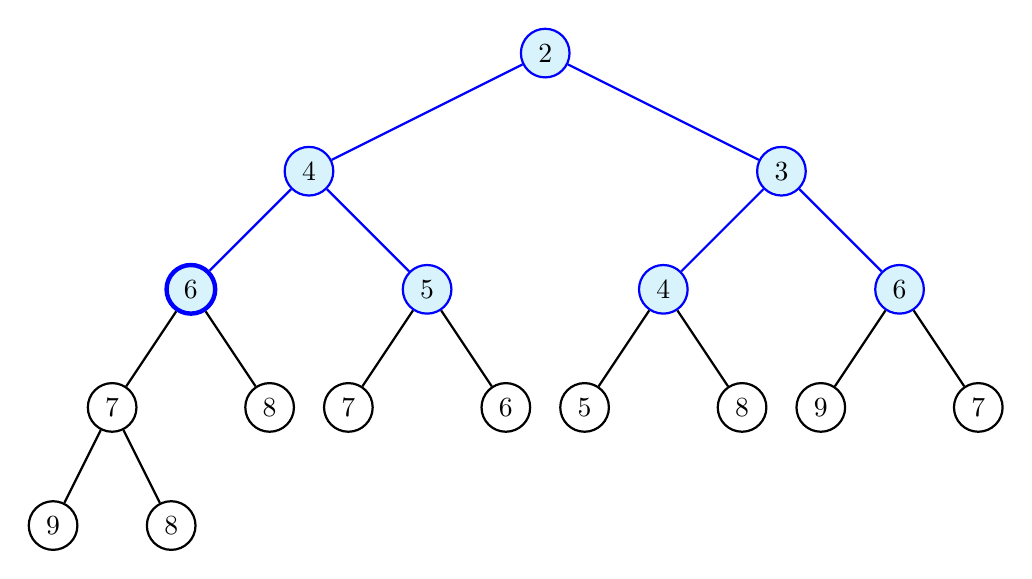
\begin{tikzpicture}[level/.style={sibling distance=60mm/#1}]
		\node [circle,thick,draw=blue,fill=cyan!15] (0) {2}
		child[thick,draw=blue] { node [circle,draw,fill=cyan!15] (1) {4}
			child { node [circle,draw,ultra thick,fill=cyan!15] (3) {6}
				child[draw=black] { node [circle,draw] (7) {7} 
					child { node [circle,draw] (15) {9} }
					child { node [circle,draw] (16) {8} }				
				}
				child[draw=black] { node [circle,draw] (8) {8} }
			}
			child { node [circle,draw,fill=cyan!15] (4) {5}
				child[draw=black] { node [circle,draw] (9) {7} }
				child[draw=black] { node [circle,draw] (10) {6} }
			}
		}
		child[thick,draw=blue] { node [circle,draw,fill=cyan!15] (2) {3}
			child { node [circle,draw,fill=cyan!15] (5) {4}
				child[draw=black] { node [circle,draw] (11) {5} }
				child[draw=black] { node [circle,draw] (12) {8} }
			}
			child { node [circle,draw,fill=cyan!15] (7) {6}
				child[draw=black] { node [circle,draw] (13) {9} }
				child[draw=black] { node [circle,draw] (14) {7} }
			}
		};
	\end{tikzpicture}
	\caption{Ukázka vrchního řezu haldy pomocí rodiče}\label{img:heap-upper-parent-cut}
\end{figure}

\begin{remark}
	V grafu vrchního řezu haldy pomocí rodiče platí haldové uspořádání.
\end{remark}

\begin{definition}[Spodní řez haldy pomocí rodiče]
	Mějme graf $G = (V, E)$ reprezentující binární haldu a~$i \in \mathbb{N}$.
	Spodním řezem haldy pomocí rodiče nazveme graf $G' = (V', E')$, kde
	\begin{enumerate}
	  \item[] $V' = \{ v: v \in V \land \Index(v) > i \}$
	  \item[] $E' = \{ (u, v): (u, v) \in E \land u \in V' \land v \in V' \}$.
	\end{enumerate}
\end{definition}

\begin{figure}[H]
	\centering
	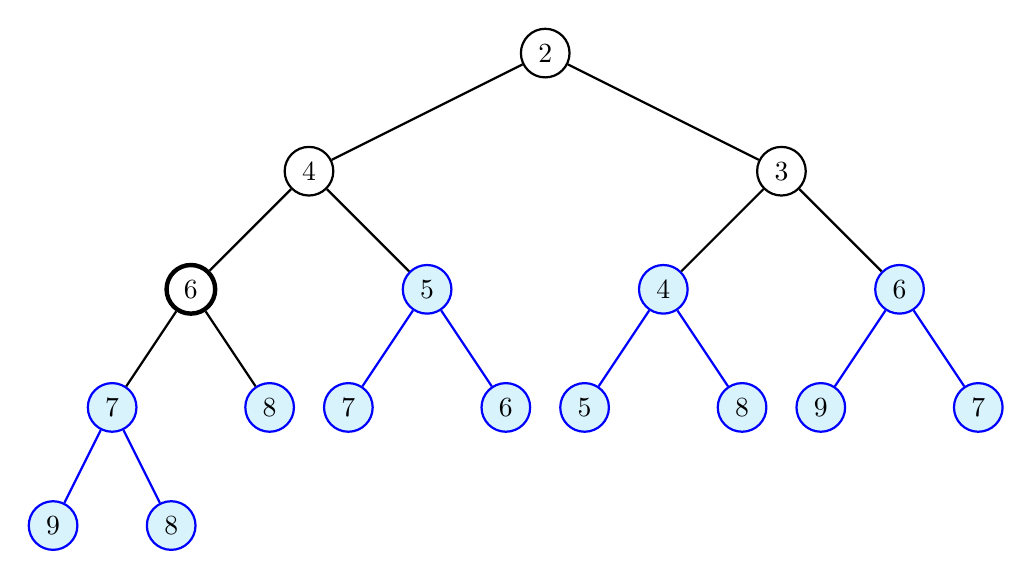
\begin{tikzpicture}[level/.style={sibling distance=60mm/#1}]
		\node [circle,draw,thick] (0) {2}
		child[thick] { node [circle,draw] (1) {4}
			child { node [circle,draw,ultra thick] (3) {6}
				child { node [circle,draw=blue,fill=cyan!15] (7) {7} 
					child[draw=blue] { node [circle,draw,fill=cyan!15] (15) {9} }
					child[draw=blue] { node [circle,draw,fill=cyan!15] (16) {8} }				
				}
				child { node [circle,draw=blue,fill=cyan!15] (8) {8} }
			}
			child { node [circle,draw=blue,fill=cyan!15] (4) {5}
				child[draw=blue] { node [circle,draw,fill=cyan!15] (9) {7} }
				child[draw=blue] { node [circle,draw,fill=cyan!15] (10) {6} }
			}
		}
		child[thick] { node [circle,draw] (2) {3}
			child { node [circle,draw=blue,fill=cyan!15] (5) {4}
				child[draw=blue] { node [circle,draw,fill=cyan!15] (11) {5} }
				child[draw=blue] { node [circle,draw,fill=cyan!15] (12) {8} }
			}
			child { node [circle,draw=blue,fill=cyan!15] (7) {6}
				child[draw=blue] { node [circle,draw,fill=cyan!15] (13) {9} }
				child[draw=blue] { node [circle,draw,fill=cyan!15] (14) {7} }
			}
		};
	\end{tikzpicture}
	\caption{Ukázka spodního řezu haldy pomocí rodiče}\label{img:heap-lower-parent-cut}
\end{figure}

\begin{remark}
	V grafu spodního řezu haldy pomocí rodiče platí haldové uspořádání.
\end{remark}

\begin{listing}[H]
	\caption{Probublání prvku dolů}
	\label{list:bubbledown}
	\begin{minted}{c}
void HeapBubbleDown(Heap heap, int index) {
  int child;

  while (HeapHasChild(heap, index)) {
    child = HeapLowerChild(heap, index);

    if (HeapElementValue(heap, index) <= HeapElementValue(heap, child)) {
      break;
    }

    HeapSwap(heap, index, child);

    index = child;
  }
}
	\end{minted}
\end{listing}



\section{Odstranění minimálního prvku}

\section{Změna hodnoty vrcholu}

\subsection{Snížení hodnoty vrcholu}

\subsection{Zvýšení hodnoty vrcholu}

\section{Konstrukce haldy}


%---------------------------------------------------------------
\chapter{Metody ladění při vývoji důkazu}
%---------------------------------------------------------------

\section{Zúžení vstupních podmínek}

\section{Krokování}

\section{Kontradikce}



%\section{Důkazy s referenčními datovými typy}
%
%V průběhu tvorby autor práce předával datovou strukturu mezi jednotlivými funkcemi pomocí odkazu na paměť. Princip předávání celé datové struktury pomocí odkazu umožňuje minimalizovat počet proměnných na zásobníku a všechny hodnoty ukládá v dynamické části paměti.
%
%Datová struktura reprezentující haldu se sestává z ukazatele na začátek pole, ve kterém jsou prvky haldy uložené, celočíselné hodnoty reprezentující aktuální počet uložených prvků v haldě a maximální kapacitu alokované paměti pole.
%
%Pokud je tato struktura předaná do některé obslužné funkce, která by s některými hodnotami pracovala, Frama-C a její WP plugin nemůže zajistit, že se v průběhu provádění dané funkce hodnoty nebudou měnit. Jelikož k hodnotám uloženým v haldě přistupujeme pomocí dereference ukazatele, může se teoreticky kdykoli stát, že hodnoty v paměti, kam daný ukazatel ukazuje již nejsou aktuální. Příkladem můžou být například vícevláknové aplikace.
%
%\section{Opravení haldy probubláním nahoru}
%
%Probublání prvku nahoru potřeba provést, pokud se v některý moment objeví v haldě prvek, který nesplňuje vlastnosti haldy a hodnota v daném vrcholu je menší, než hodnota v jeho rodiči. Tento stav nastává při vkládání prvku do haldy, kde se nový prvek přidá jako poslední prvek v téměř úplném binárním stromě a provede se probublání nahoru, aby se daný prvek dostal do správného místa v haldě tak, aby byla zajištěna vlastnost haldy pro všechny vrcholy rodičů a jejich synů.
%
%\subsection{Řez haldou}
%
%Pro důkaz autor využil řez haldou, který rozděluje graf haldy dle vlastnosti haldy (hodnota v rodiči je menší nebo rovna hodnotám v jeho synech) na dvě části. Korektní halda splňuje haldovu vlastnost mezi všemi dvojicemi rodič - syn. 
%Vrchní řez haldou tento predikát omezuje pouze na syny, kteří mají index v haldě ostře menší než problematický vrchol. Pro tyto vrcholy a jejich rodiče musí platit haldová vlastnost.
%Spodní řez haldou omezuje původní predikát na vrcholy, které mají index v haldě ostře větší než problematický index a pro ně také musí platit haldová vlastnost.
%Pro algoritmus probublání nahoru musí být zajištěno, že pouze problematický vrchol jakožto syn může porušovat haldoovu podmínku se svým rodičem.
%Princip důkazu spočívá v postupném posouvání vrchního a horního řezu do té doby, než horní řez není aplikován na žádný vrchol a spodní řez je aplikován na celou haldu. Tento moment nastává při pokusu o probublání kořene haldy. Jelikož žádný syn nemůže mít menší vrchol než kořen, predikát horního řezu je triviálně splněn. Dolní řež je poté speciálním případem původního predikátu korektní haldy. Tento princip je také zefektivněn v případě, že najdeme správné místo, kde by měl problematický vrchol zůstat, haldová vlastnost určitě platí pro vrcholy v horním i spodním řezu a nově i pro správně probublaný vrchol, což zaručuje plně splněný původní predikát korektní haldy.
%
%\section{Důkaz korektnosti algoritmu opravení haldy probubláním dolů}
%
%Podobně jako v případě probublání problémového prvku nahoru je u algoritmu probublání prvku haldy dolů využit řez haldou. Oproti řezu, který byl využit pro probublání nahoru tento řez mluví o rodičích. Protože v případě problémového prvku je možné, že pro oba jeho syny bude potrebušena haldová vlastnost. Kdežto pří probublání nahoru bylo přímo jasné mezi kterou dvojicí rodič syn je vlastnost porušená.



\inputminted{c}{code/reference-problematic.c}

\begin{minted}{c}
/*@
    requires ...;
*/
void HeapInsert(Heap *heap)
{
    // ...
}
\end{minted}

\lipsum[2] \cite{def:1, def:2}

%---------------------------------------------------------------
\chapter{Hledání nejkratší cesty}
%---------------------------------------------------------------

\section{Dijkstrův algoritmus}

%---------------------------------------------------------------
\chapter{Vývojové prostředí}
%---------------------------------------------------------------

\section{Docker}

\subsection{Reverzní proxy}

\subsection{Editor kódu}

\subsection{Verifikační prostředí}


\subsection{Class aptent taciti}

\lipsum[2-3]

\begin{description}
\item[Kapitola 1] Lorem ipsum dolor sit amet, consectetuer adipiscing elit. Curabitur sagittis hendrerit ante. Class aptent taciti sociosqu ad litora torquent per conubia nostra, per inceptos hymenaeos. Cras pede libero, dapibus nec, pretium sit amet, tempor quis.

\item[Kapitola 2] Lorem ipsum dolor sit amet, consectetuer adipiscing elit. Curabitur sagittis hendrerit ante. Class aptent taciti sociosqu ad litora torquent per conubia nostra, per inceptos hymenaeos. Cras pede libero, dapibus nec, pretium sit amet, tempor quis.

\item[Kapitola 3] Lorem ipsum dolor sit amet, consectetuer adipiscing elit. Curabitur sagittis hendrerit ante. Class aptent taciti sociosqu ad litora torquent per conubia nostra, per inceptos hymenaeos. Cras pede libero, dapibus nec, pretium sit amet, tempor quis.

\item[Kapitola 4] Lorem ipsum dolor sit amet, consectetuer adipiscing elit. Curabitur sagittis hendrerit ante. Class aptent taciti sociosqu ad litora torquent per conubia nostra, per inceptos hymenaeos. Cras pede libero, dapibus nec, pretium sit amet, tempor quis.
\end{description}

\lipsum[2]

\section{Lorem ipsum dolor sit amet}

\lipsum[3-5]
